One way to provide Internet access is by connecting the \gls{mp} with an Ethernet cable to the jack port in the wall. The Mesh Potato is delivered pre-configured, with the IP address and the name of the network (SSID) stated in the "Get Started - How to Use the Box"-document included in the \gls{quick} box. \fref{fig:oppsettfraveggen} illustrates how the components are connected together in the following manual. The figure is provided to help the user get a better understanding of the network.  

\begin{figure}[h!]
  \centering
      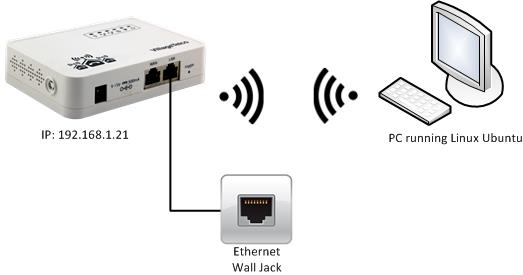
\includegraphics[width=0.78\textwidth]{oppsettfraveggen}
  \caption [How the components are linked together during set-up for accessing the Internet from wall jack]{\textbf{How the components are linked together during set-up for accessing the Internet from wall jack.} This figure shows how the different components are set up when the manual for providing Internet access from a wall jack is carried out. As shown, the PC is connected to the MP via WiFi in order to perform the configurations on the MP.}
  \label{fig:oppsettfraveggen}
\end{figure}



\begin{enumerate}
\item Do the following steps to connect the PC via WiFi to the \gls{mp}:
\begin{enumerate}
\item Press the WiFi symbol in the top right corner of your Linux Ubuntu home screen, and press "Edit Connections".
\item  Under the tab "Wireless" choose the network called "vt-mesh" and press "Edit" like shown in \fref{fig:networkconnections}.
\begin{figure}[h!]
  \centering
      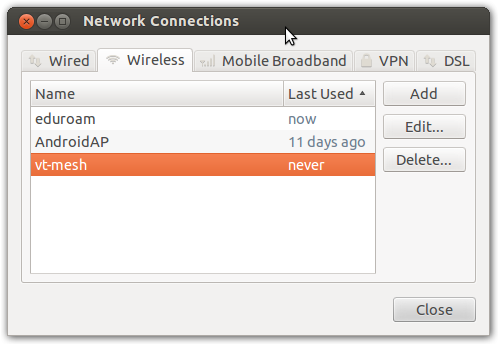
\includegraphics[width=0.7\textwidth]{networkconnections.PNG}
  \caption [Network Connections on Linux Ubuntu]{\textbf{This figure shows the "vt-mesh" under Wireless Network Connections.}}
  \label{fig:networkconnections}
\end{figure}

\item In the field "BSSID" enter "02:CA:FF:EE:BA:BE", like shown in \fref{fig:bssid}.
\item Under the tab "IPv4 Settings" choose "Manual" in the "Method" drop-down menu, like shown in \fref{fig:ipv4settings}. 
\item Then press "Add" on the same page. Enter the following parameters, like shown in \fref{fig:ipv4settings}:
\begin{description}
\item[] \textbf{Address:} 10.10.1.245
\item[] \textbf{Netmask:} 24
\item[] \textbf{Gateway:} 10.130.1.1
\end{description}
\begin{figure}[h!]
        \centering
        \begin{subfigure}[t]{0.49\textwidth}
                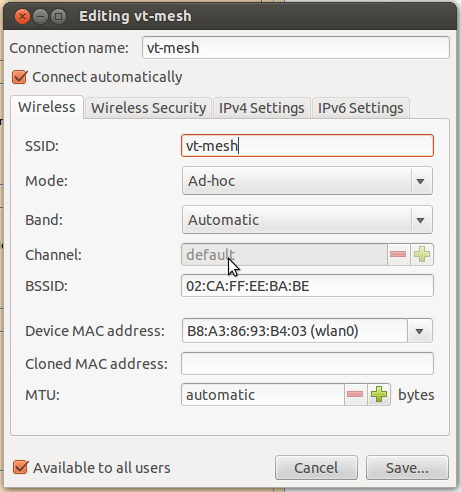
\includegraphics[width=\textwidth]{bssid.PNG}
                \caption{\textbf{The correct BSSID set.}}\label{fig:bssid}
        \end{subfigure}
        \begin{subfigure}[t]{0.49\textwidth}
                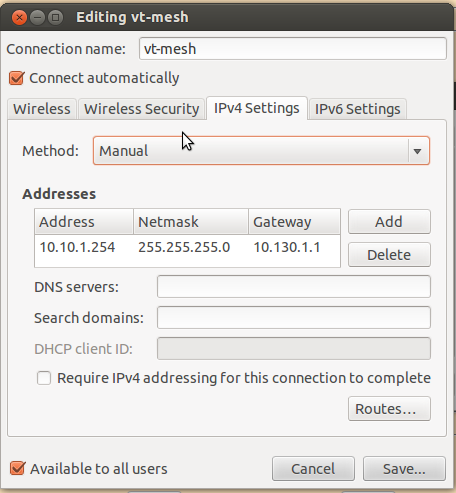
\includegraphics[width=\textwidth]{ipv4settings.PNG}
                \caption{\textbf{The correct parameters set under IPv4 settings.}}\label{fig:ipv4settings}
        \end{subfigure}
\caption{"Edit Connections" settings on Linux}
\end{figure}
\item Press "Save" on the "Editing vt-mesh"-window, and then "Close" on the "Network Connections"-window. 
\item Then choose "vt-mesh" from the list of available networks. This list is found after pressing the WiFi symbol in the top right corner on your screen. The PC should then be connected to the MP via WiFi. 
\end{enumerate}
\item Connect an Ethernet cable from the LAN-port on the MP (make sure the MP is powered up) to the wall jack (cabled Internet).
\item Open the terminal window on the PC by pressing "Ctrl+Alt+t" and type in the following commands to telnet into the \gls{mp}:
\noindent
\begin{lstlisting}[language=bash]
  $ sudo su
  $ telnet 10.10.1.20
\end{lstlisting}
We highly recommend that you enhance the security on the \gls{mp} by enabling SSH instead of telnet. This has no impact on this set-up, and will not affect the ability to provide Internet access to the network. Description on how to enable SSH is found in section \ref{subsubsec:ssh}.
\item To verify that the previous command was executed correctly, a "picture" will appear in your terminal saying "Welcome to Village Telco". Execute the following command to finish the set-up:
\noindent
\begin{lstlisting}[language=bash]
 $ udhcpc -i br-lan
\end{lstlisting}
\item A "Sending discover ..." appears, and a lease is obtained like shown in \fref{fig:sendingdiscover}. 
\begin{figure}[h!]
  \centering
      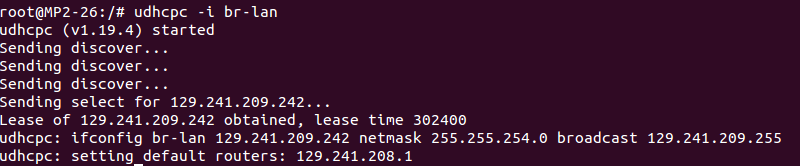
\includegraphics[width=1\textwidth]{sendingdiscover.PNG}
  \caption [The results from executing "uchcpc -i br-lan".]{\textbf{This figure shows the allocation of lease after executing "uchcpc -i br-lan".}}
  \label{fig:sendingdiscover}
\end{figure}
\item After the lease is obtained, the \gls{mp} is provided with Internet access. You can test this by connecting to the \gls{mp} from, for example, your smart phone or a PC. 
\begin{itemize}
\item The name of the network: \textbf{MP2_21}
\item The password is: \textbf{potato-potato}
\end{itemize}
Both the name and the password can be changed in the web interface. 
\end{enumerate}
